% !TeX root = ../main.tex
\section{Kinetics Parameters}
\label{app:kinetics}

%\subsection{Summary of production routes}

% 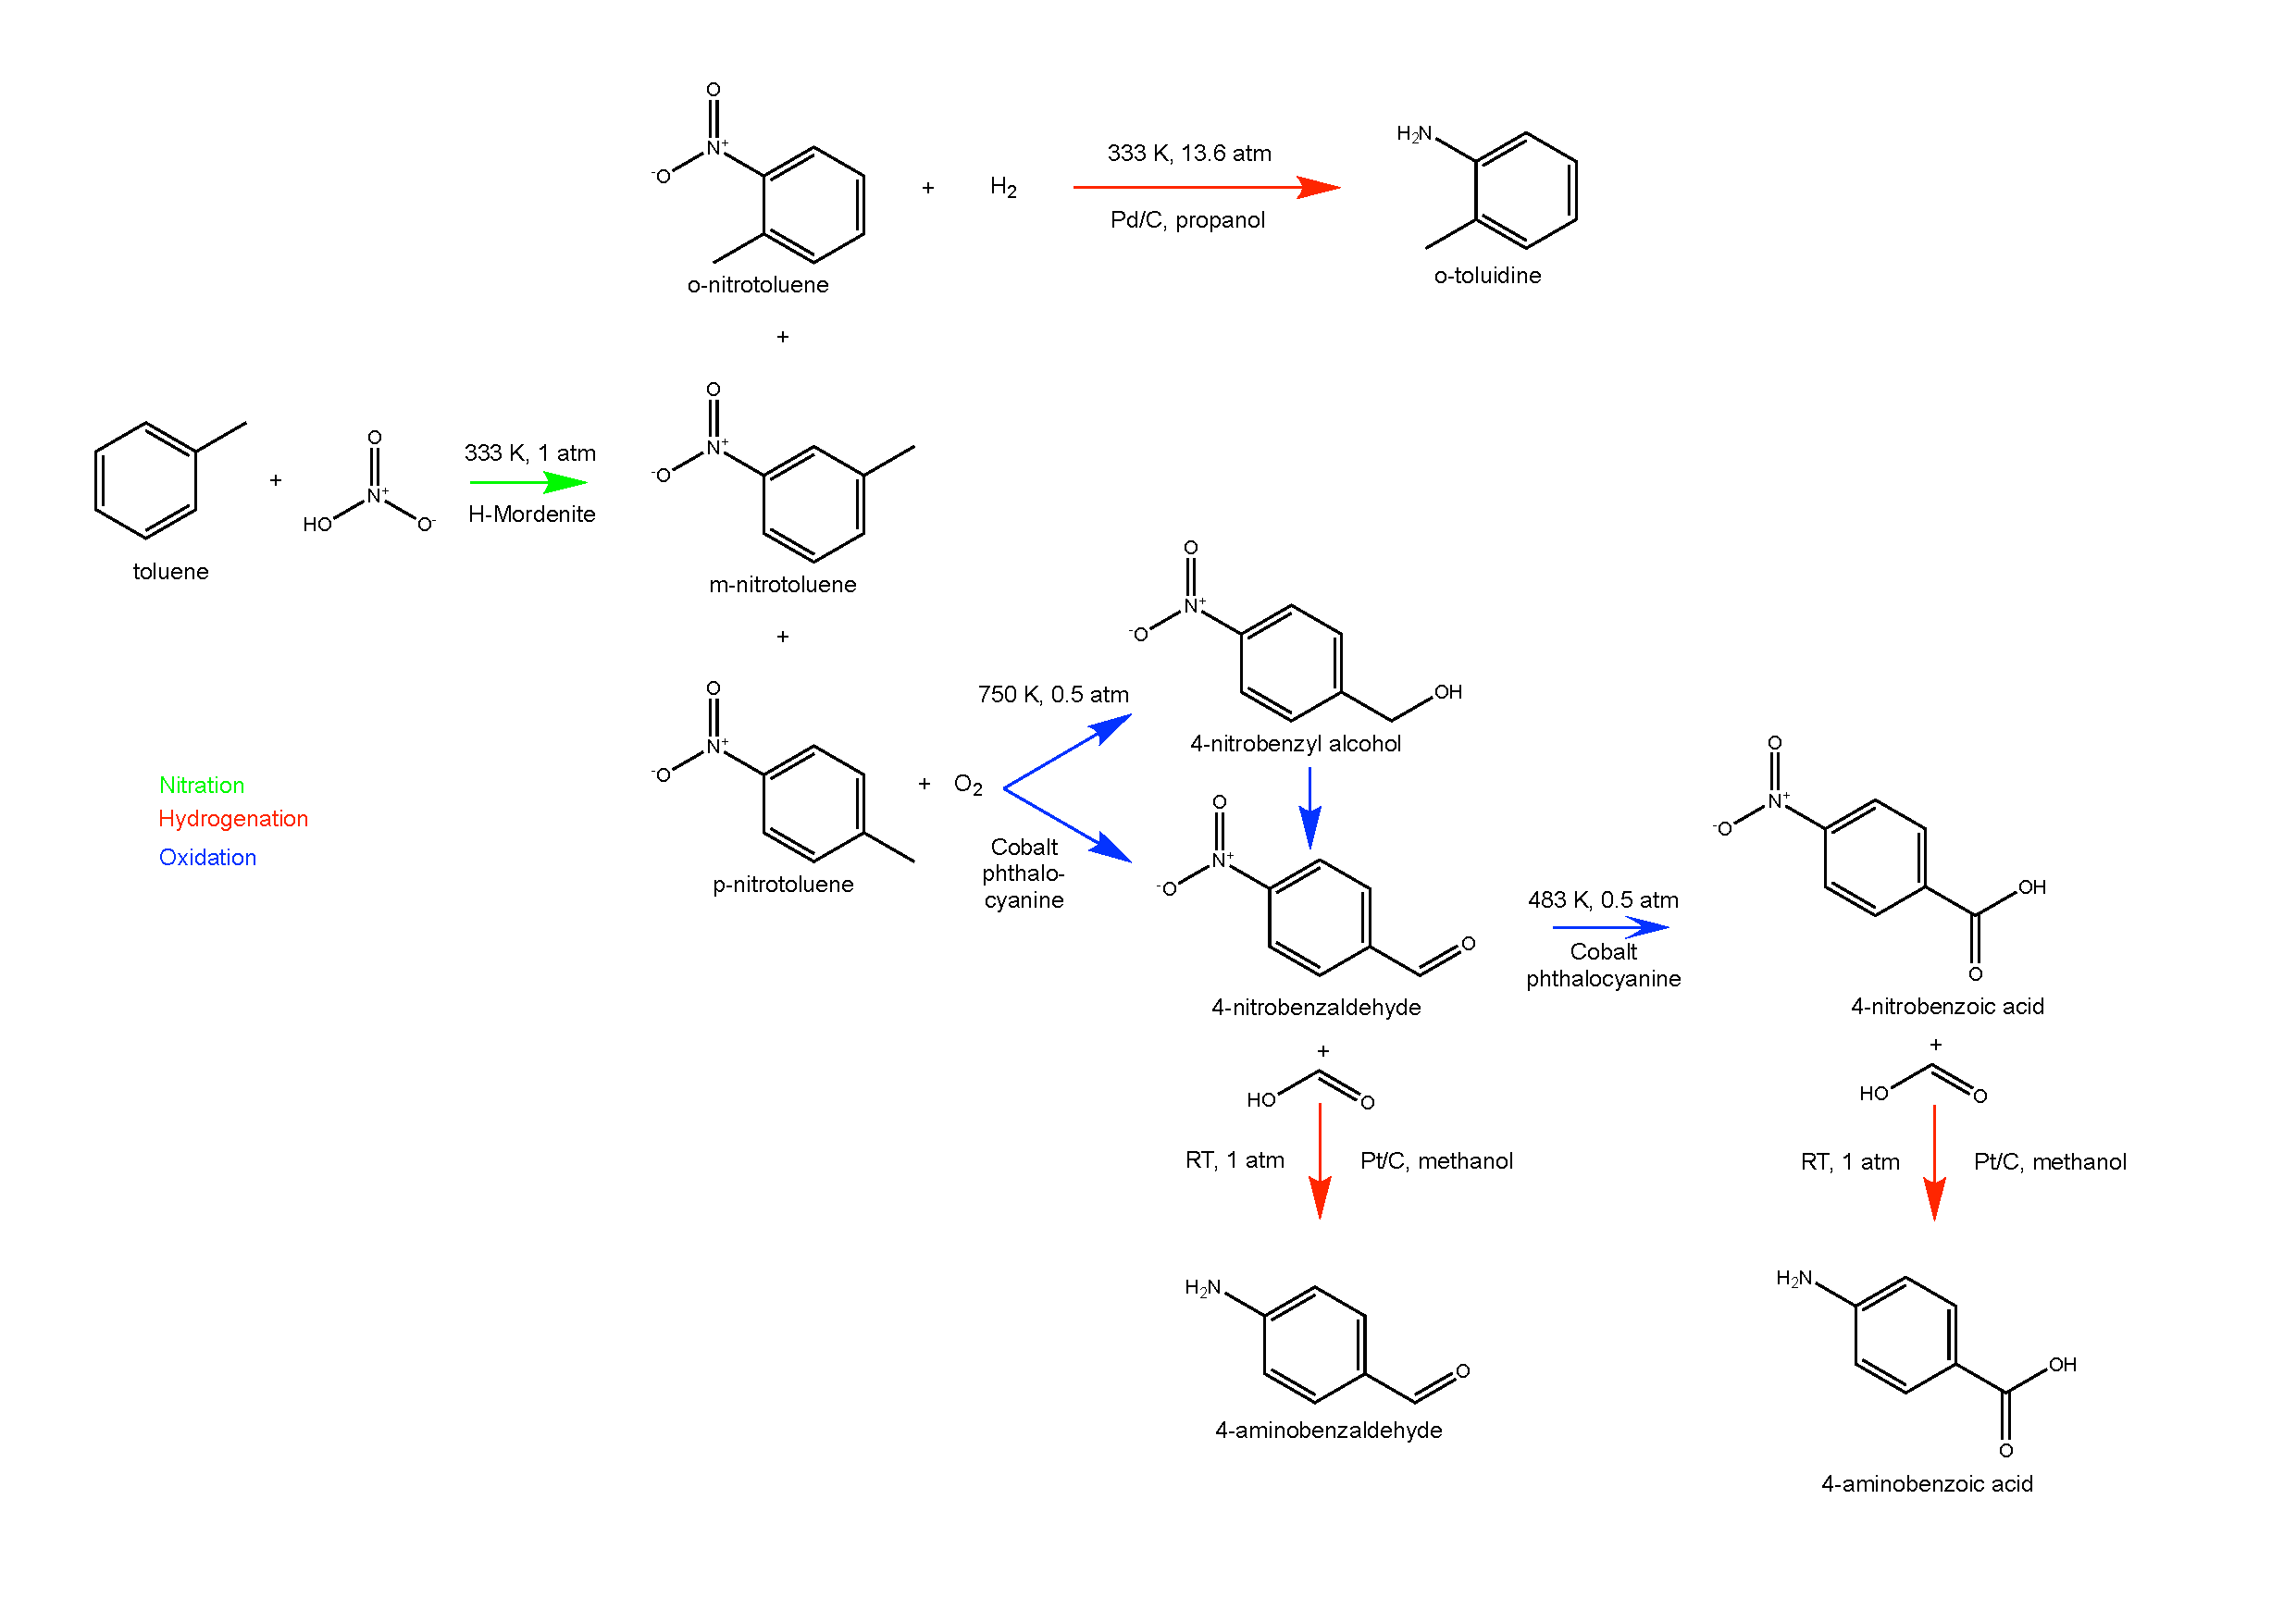
\includepdf[pages=-,landscape]{figures/routes-chosen.pdf}

\afterpage{
\begin{landscape}
\begin{figure}[H]
    \centering
    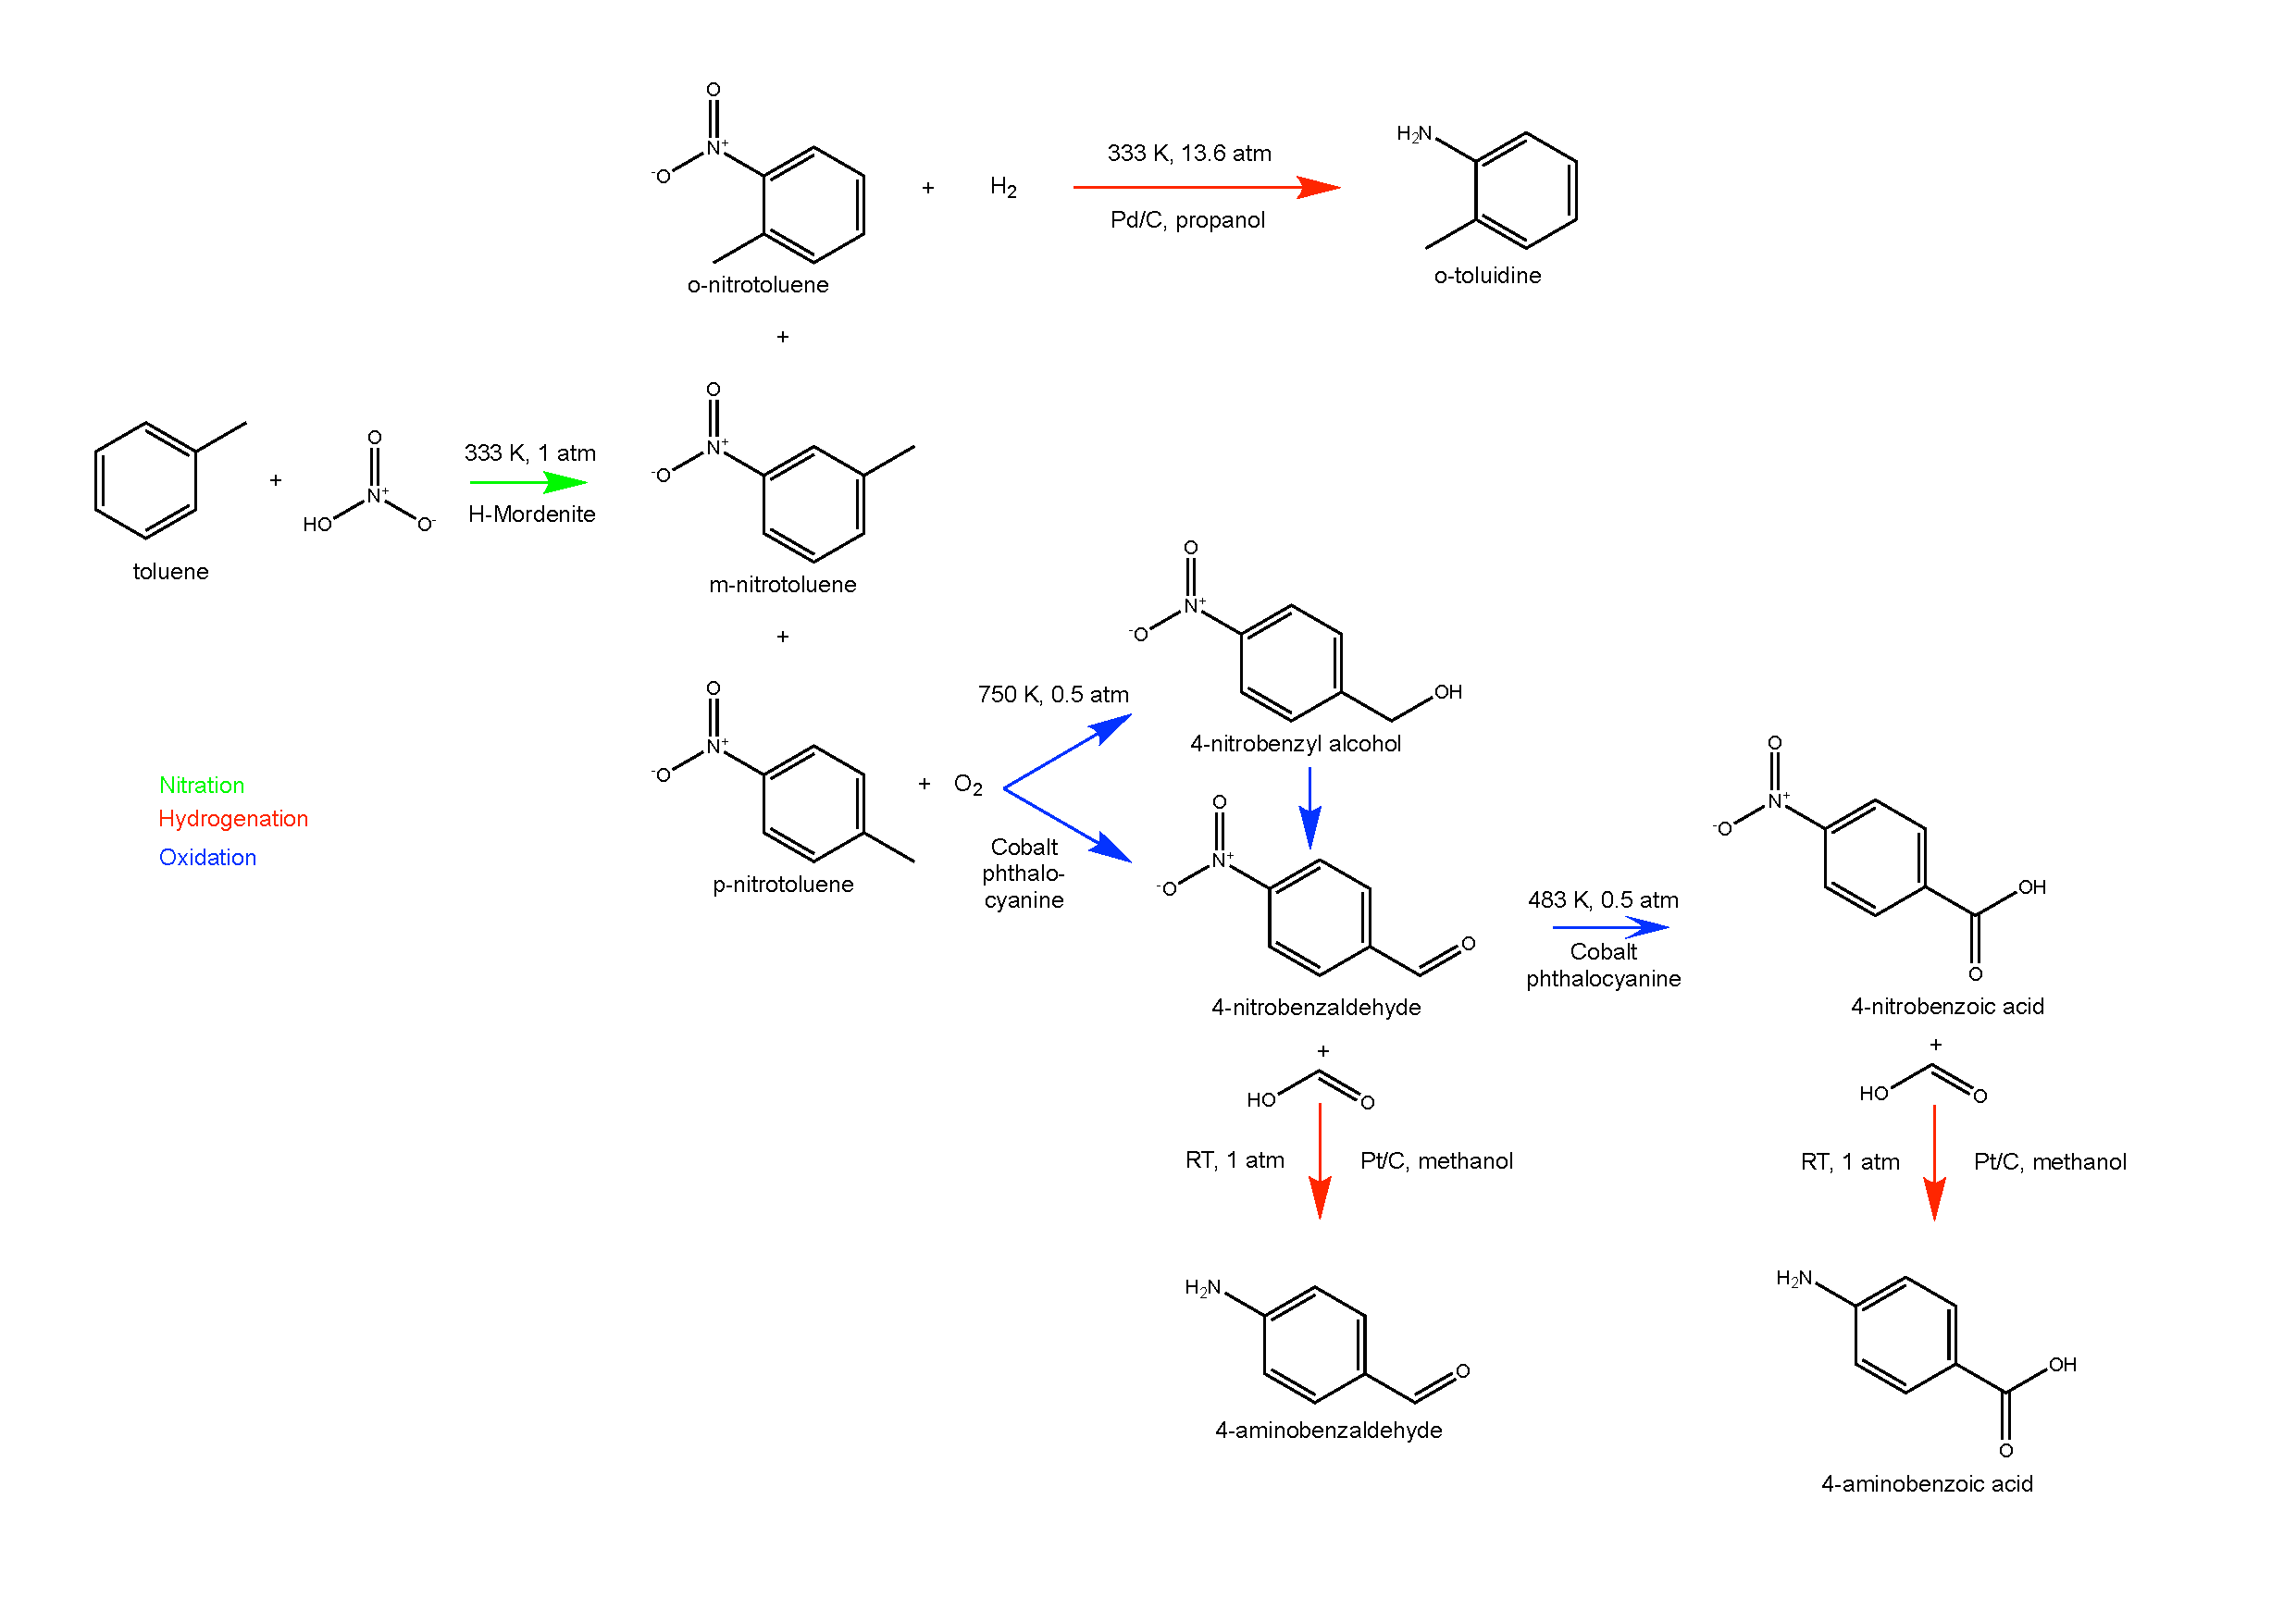
\includegraphics[width=0.8\linewidth]{figures/routes-chosen.pdf}
    \caption{Selected synthesis routes}
    \label{fig:routes-chosen}
\end{figure}
\end{landscape}
}

\subsection{Toluene nitration}
\paragraph{Assumptions}
\begin{itemize}
    \item The stoichiometric reaction is \ch{Toluene +  HNO3 -> 0.44 PNT + 0.03 MNT + 0.53 ONT + H2O}, where PNT, MNT and ONT are respectively the \textit{para}, \textit{meta} and \textit{ortho} isomers of nitroltoluene.
    \item The ratio of isomers is reflected in the stoichiometric eqution \cite{smith_novel_1998}.
    \item Negligible production of dinitrotoluene by-products as reported selectivity with H-Mordenite catalyst is lower than 0.55mol\% \cite{jeeru_kinetics_2018}.
    \item Kinetic parameters were obtained for a system free from mass transfer resistances and thus when the reaction is kinetically controlled \cite{jeeru_kinetics_2018}. Hence we can safely assume that the intrinsic rate of reaction was measured.
    \item The rate of reaction of toluene is first order in toluene and nitric acid concentrations. However with 2:1 mole ratio of nitric acid to toluene, the rate can be approximated to a pseudo-first order reaction with respect to toluene \cite{jeeru_kinetics_2018}.
    \begin{equation}
    - \frac{dC_{toluene}}{dt}=k \cdot C_{toluene} 
    \end{equation}
    \item The rate constant follows the Arrhenius law below, which is valid for a reaction temperature range of 303-363K \cite{jeeru_kinetics_2018}:
    \begin{equation}
        k=2.5e^{-\frac{24.24\cdot 10^{3}}{RT}}
    \end{equation}
    \item The loss in activity of the catalyst can be neglected \cite{jeeru_kinetics_2018}.
\end{itemize}

\subsection{o-nitrotoluene hydrogenation}
\paragraph{Assumptions}
\begin{itemize}
    \item The stoichiometric reaction is \ch{ONT +  3 H2 -> \ortho-toluidine + 2 H2O} [].
    \item Negligible production of dinitrotoluene by-products as reported selectivity with H-Mordenite catalyst is lower than 0.55mol\% \cite{jeeru_kinetics_2018}.
    \item Kinetic parameters were obtained for a system free from mass transfer resistances and thus when the reaction is kinetically controlled \cite{jeeru_kinetics_2018}. Hence we can safely assume that the intrinsic rate of reaction was measured.
    \item The rate of reaction of toluene is first order in toluene and nitric acid concentrations. However with 2:1 mole ratio of nitric acid to toluene, the rate can be approximated to a pseudo-first order reaction with respect to toluene \cite{jeeru_kinetics_2018}.
    \begin{equation}
    - \frac{dC_{toluene}}{dt}=k \cdot P_{\ch{H2}}^{0.3} 
    \end{equation}
    \item The rate constant, in \mol\per\kPa$^{3}$\g$_{cat}$\s, is valid for a reaction temperature range of 303-363K \cite{sol}:
    \begin{equation}
        k=1852e^{\frac{-45.52\cdot 10^{3}}{RT}}
    \end{equation}
    \item The loss in activity of the catalyst can be neglected \cite{}.
\end{itemize}

\subsection{4-nitrotoluene oxidation}
\paragraph{Assumptions}
\begin{itemize}
    \item 
\end{itemize}

\subsection{Reduction of 4-nitrobenzaldehyde and 4-nitrobenzoic acid}
\paragraph{Assumptions}
\begin{itemize}
    \item The stoichiometric reaction is \ch{R-NO2 + !( formic~acid )( HCOOH ) ->['\SI{5}{\percent}' Pt/C] R-NH2 + CO2 + O2}
\end{itemize}
